% ============================================================================
% Geophysical Research Letters (AGU) manuscript
% Requires the AGU class agujournal2019.cls + apacite (from the AGU LaTeX
% template zip or the Overleaf "AGU" gallery). An Overleaf AGU project can be
% transferred straight to the GRL submission system (see AGU LaTeX guidelines).
% If agujournal2019.cls is unavailable, a plain-article shim is described in
% README-grl.md for local proof-compiling only.
% Compile: pdflatex -> bibtex -> pdflatex -> pdflatex
% ----------------------------------------------------------------------------
% GRL limits: <=12 publication units [PU = words/500 + figs + tables];
% abstract <150 words; 3 Key Points (<=140 chars each); Plain Language Summary.
% This file: 4 figures + 1 table (= 5 PU) in main text; everything else is in
% the Supporting Information (moho-indonesia-grl-si.tex).
% ============================================================================
\documentclass{agujournal2019}
\usepackage{url}
\usepackage{lineno}
\linenumbers
\draftfalse

\journalname{Geophysical Research Letters}

\begin{document}

\title{The Moho of Indonesia from Satellite Gravity: A Fast Spherical Inversion
Validated Against Seismic Estimates and Global Crustal Models}

\authors{Muhammad Zuhdi\affil{1}, Sudarmaji\affil{1}, and Wiwit Suryanto\affil{1}}
\affiliation{1}{Geophysics Laboratory, Department of Physics, Universitas Gadjah
Mada, Sekip Utara PO BOX BLS 21, Yogyakarta 55281, Indonesia}
\correspondingauthor{Wiwit Suryanto}{ws@ugm.ac.id}

\begin{keypoints}
\item First continuous satellite-gravity Moho model for the whole Indonesian
archipelago, from a fast spherical Bott--Tikhonov inversion
\item It fits 105 receiver-function Moho depths to 5.8~km and agrees with seismic
AusMoho at the Australian margin (bias $-0.1$~km, $r=0.86$)
\item It equals CRUST1.0 at the seismic points, whereas GOCE-derived GEMMA is
$\sim$7~km too shallow, showing global models are inadequate here
\end{keypoints}

\begin{abstract}
Moho depth across the Indonesian archipelago is known only unevenly, from sparse
seismic stations. We estimate it from satellite gravity using the fast,
regularized, spherical tesseroid inversion of Uieda and Barbosa (2017), which
inverts the anomalous Moho with Bott's method stabilized by Tikhonov
regularization. Gravity disturbances from the satellite-only model GOCO06s are
corrected for topography and bathymetry, and hyperparameters are set by
cross-validation and 105 receiver-function Moho depths. The preferred model fits
the seismic Moho to a mean of $+1.2$~km and standard deviation of $5.8$~km, and
agrees with the independent seismic AusMoho model along the northern Australian
margin (bias $-0.1$~km, $r=0.86$). At the seismic stations the model equals
CRUST1.0 despite five-times-finer resolution, whereas GOCE-derived GEMMA is
systematically $7.4$~km too shallow. The Moho thickens beneath the arcs and
collision belts and thins beneath the marginal basins, tracking the region's
tectonics.
\end{abstract}

\section*{Plain Language Summary}
The Moho is the boundary between Earth's crust and mantle; its depth reveals where
the crust is thick or thin and underpins studies of earthquakes and volcanoes.
Across Indonesia, one of the most tectonically active regions on Earth, this depth
is measured only near scattered seismic stations, leaving most of the vast
archipelago and its seas unmapped. Satellite gravity, by contrast, covers the
whole region uniformly, including offshore. We convert satellite gravity into a
map of Moho depth using an efficient method that properly accounts for Earth's
curvature, and we tune and test it with 105 independent seismic measurements. Our
map matches the seismic values as closely as the widely used global model
CRUST1.0, even though our map is five times more detailed, and it clearly
outperforms GEMMA, a global model derived purely from gravity, which is about
seven kilometres too shallow over Indonesia. The resulting map shows thick crust
beneath the volcanic arcs and mountain belts and thin crust beneath the ocean
basins, providing a consistent, openly available starting framework for crustal
and hazard studies across Indonesia.

\section{Introduction}
The Mohorovi\v{c}i\'{c} discontinuity (Moho) separates crust from mantle and is a
first-order constraint on lithospheric structure, isostasy and geodynamics. In
Indonesia --- where the Indo-Australian, Sunda, Philippine Sea and Pacific plates
interact through subduction, collision and back-arc spreading --- Moho depth
varies strongly over short distances. Seismic methods give the most direct
estimates but are limited to the vicinity of stations, concentrated on land and
along the volcanic arc \cite{zhang2023}.

Two global crustal models are used where local data are absent. CRUST1.0
\cite{laske2013} is a $1^{\circ}$ compilation that, over Indonesia, is
interpolated from sparse controls; GEMMA \cite{reguzzoni2015,rossi2022} is a
$0.5^{\circ}$ Moho inverted globally from GOCE gravity under a simplified
two-layer density model. Neither is tuned to Indonesian data, and both are too
coarse to resolve the sharp arc/fore-arc crustal contrasts of the archipelago. A
dedicated, regionally calibrated gravity Moho is therefore warranted.

Gravity provides continuous, homogeneous coverage, especially offshore. Estimating
the Moho from gravity is a nonlinear, ill-posed problem; \citeA{uieda2017}
introduced an efficient solution in \emph{spherical} coordinates combining Bott's
\cite{bott1960} iteration, tesseroid forward modelling \cite{uieda2016} and
first-order Tikhonov regularization, and applied it to South America. We transfer
that method, unchanged in principle, to the whole of Indonesia, and validate the
result against an independent seismic compilation, the seismic AusMoho model
\cite{kennett2011}, and the two global models above.

\section{Data and Methods}
We use the satellite-only global gravity model GOCO06s \cite{kvas2021} synthesised
to spherical-harmonic degree/order 300 on a regular grid at 4~km constant height,
and, as a higher-resolution variant, the altimetry free-air anomaly
\cite{sandwell2014}. Earth relief is from SRTM15+ \cite{tozer2019}. Validation uses
an independent compilation of 105 receiver-function (RF) Moho depths
($96.3^{\circ}$--$140.7^{\circ}$E, $10.2^{\circ}$S--$5.2^{\circ}$N; depths
20--40~km, mean 30.4~km; 31 on Sumatra, 24 on Java, 50 in eastern Indonesia, none
offshore; Table~S1, Figure~\ref{fig:compare}a). The most comprehensive comparable
compilation is \citeA{zhang2023}.

The gravity disturbance is $\delta = g - \gamma$, the GOCO06s gravity minus the
closed-form WGS84 normal gravity, and contains only anomalous-mass effects. All
mass effects are forward modelled with tesseroids (spherical prisms) that honour
Earth curvature \cite{uieda2016}. Removing the topographic/bathymetric effect
(land density $2670$, ocean contrast $-1640$~kg\,m$^{-3}$) gives the Bouguer
disturbance $\delta_{bg}$, the inversion input. The anomalous Moho is one tesseroid
per grid cell between the reference depth $z_{\mathrm{ref}}$ and the true depth
$z_k$, with contrast $-\Delta\rho$ where the Moho is deeper than $z_{\mathrm{ref}}$
and $+\Delta\rho$ where shallower \cite{uieda2017}.

We minimise the regularized goal function
$\Gamma(\mathbf{p}) = \|\mathbf{d}^{o}-\mathbf{d}(\mathbf{p})\|^{2}
 + \mu\,\|\mathbf{R}\mathbf{p}\|^{2}$,
where $\mathbf{p}$ are the Moho depths, $\mathbf{R}$ the first-difference operator
and $\mu$ the regularization weight. Following \citeA{bott1960} and
\citeA{silva2014}, the dense Jacobian is replaced by the diagonal Bouguer-plate
form $\mathbf{A}=-2\pi G\,\Delta\rho\,\mathbf{I}$ (the minus sign: a deeper Moho
lowers gravity), so each Gauss--Newton step solves a sparse, constant,
symmetric-positive-definite system; depths are clipped to 3--70~km and iterated to
convergence. For $\mu=0$ this reduces to the classical Bott update
$\Delta z_j = [d^{o}_j - d_j]/(2\pi G\Delta\rho)$. The three hyperparameters are
set in two steps \cite{uieda2017}: $\mu$ by hold-out cross-validation, then
$(z_{\mathrm{ref}},\Delta\rho)$ against the seismic Moho (Figure~S2). Full
equations and diagnostics are in Text~S1 and Figures~S1--S2.

\section{Results}
Cross-validation selects $\mu=10^{-10}$ (essentially unregularized). The seismic
misfit decreases monotonically with $\Delta\rho$ --- a density--depth trade-off
whose raw minimum runs to unphysical contrasts --- but the fit is only weakly
sensitive over the physical range: at $z_{\mathrm{ref}}=35$~km the RMS is 6.2, 6.0,
5.9 and 5.8~km at $\Delta\rho=400,450,500,600$~kg\,m$^{-3}$. We therefore adopt a
physical $\Delta\rho=500$~kg\,m$^{-3}$ with $z_{\mathrm{ref}}=35$~km, degrading the
fit by only 0.3~km relative to 400 and independently supported by AusMoho (below).
$\Delta\rho$ is thus an \emph{effective} contrast. Bott's iteration converged in
15--20 steps.

The preferred model (Figure~\ref{fig:moho}) yields Moho depths of $\sim$7--59~km:
thick (35--45~km) beneath the Sunda, Sulawesi and Banda arcs and the Papuan
highlands, and thin (10--20~km) beneath the marginal and oceanic basins, with the
35-km contour outlining the arc/continental blocks. It differs from the 105 seismic
depths by a mean of $+1.2$~km and standard deviation of $5.8$~km
(Figure~\ref{fig:validation}), comparable to the South American result (1.2,
6.8~km); the median is $+1.2$~km, interquartile range 6.9~km, with 63\% and 89\% of
stations within $\pm5$ and $\pm10$~km. This scatter is comparable to the identical
method in South America (6.8~km; \citeA{uieda2017}) and to the seismically
referenced CRUST1.0 at these same stations (5.3~km; below), and gravity Moho models
routinely differ from seismic and from each other by 4--8~km
\cite{vandermeijde2013,reguzzoni2015}. The modest point correlation ($r=0.28$)
reflects the narrow 20--40~km range and clustering of the RF depths and a
resolution-driven amplitude compression: the smooth $\sim$67-km gravity field
underestimates the sharpest local extremes (regression slope 0.20, intercept
25~km; Figure~\ref{fig:scatter}), overestimating the thinnest and underestimating
the thickest RF crust, while tracking the mean trend (binned-mean $r=0.94$); the
seismically compiled CRUST1.0 shows the same compression at these points (slope
0.23), so the low slope reflects the reference data and scale mismatch, not our
inversion. The grid-to-grid AusMoho comparison (below), which matches like with
like, is a fairer test and yields $r=0.86$. Refining the grid to
$0.25^{\circ}$ with GOCO06s does not improve the fit, because at degree/order 300
the shortest resolved half-wavelength is $\approx67$~km; the altimetry field
recovers finer detail and near-zero bias (Table~S2).

\textbf{AusMoho.} Extending the domain south, over the northern Australian mainland
($15^{\circ}$--$11.5^{\circ}$S, $N=369$) our gravity Moho matches the independent
seismic AusMoho \cite{kennett2011} with a mean difference of $-0.1$~km, standard
deviation $4.8$~km and $r=0.86$ --- external confirmation that the method recovers
absolute depth. Crust thickens to 39--50~km at the Timor--Banda collision front.

\textbf{Global models.} Sampled at the 105 seismic stations
(Table~\ref{tab:compare}; Figures~\ref{fig:scatter}--\ref{fig:compare}), our model
matches CRUST1.0 (std 5.8 vs 5.3~km; 89\% vs 94\% within $\pm10$~km) despite being
independent and five times finer --- and although CRUST1.0 itself incorporates some
of the same RF results as priors. GEMMA, by contrast, is systematically $7.4$~km
too shallow (RMS $10.2$~km, $r=0.08$), with the largest deficits (15--24~km) at the
fore-arc/island-arc transitions of southern Java and the Banda arc, where its
coarse grid and global density model cannot capture the crustal thickening resolved
by both the seismic stations and our inversion. Spatially
(Figure~\ref{fig:compare}), our model agrees with CRUST1.0 to within $\pm5$~km in
the continental interior and diverges (deeper) mainly along the Sunda--Java trench;
it is deeper than GEMMA almost everywhere. Grid-to-grid
(Figure~\ref{fig:scatter}d--f) our model matches CRUST1.0 in amplitude (slope 0.78)
and reproduces GEMMA's spatial pattern (slope 0.93) but at a $\sim8$~km deeper,
seismically more consistent level.

\section{Discussion and Conclusions}
The gravity Moho is organized by tectonics: thick crust follows the volcanic arc
and the Sulawesi--Banda--Papua collision belts, thin crust marks the oceanic
marginal basins, and Holocene volcanoes sit along the thick-crust arc
(Figures~S3--S4). The station benchmark shows the model is competitive with the
seismically compiled CRUST1.0 and markedly better than the purely gravimetric
GEMMA, quantifying why global models are inadequate for Indonesia and motivating a
regional treatment.

Limitations follow from the method and data. Validation is land-biased and cannot
constrain the offshore Moho directly; resolution is set by the satellite gravity,
not the grid; a single, uniform $\Delta\rho$ over oceanic-to-continental crust is a
simplification; and because the diagonal Jacobian assigns all anomalous gravity to
the Moho, the subducting Sunda--Banda slabs are not separated and can deepen the
estimate near the trenches --- consistent with the deeper-than-CRUST1.0 signature
there and with the largest residuals at the subduction fronts. We give a
sensitivity-based error bound rather than a formal uncertainty map: across
$\Delta\rho=400$--$600$~kg\,m$^{-3}$ the seismic RMS moves by $<0.5$~km, and the
$5.8$~km scatter is an empirical error at the stations. A CRUST1.0 sediment
correction did not improve the fit (Text~S1). Dedicated offshore refraction
profiles \cite{planert2010} would provide direct marine control.

We produced the first continuous, public-data, satellite-gravity Moho model for the
whole Indonesian region. Calibrated against 105 seismic depths and cross-checked
against AusMoho, CRUST1.0 and GEMMA, it reproduces first-order crustal-thickness
variations, fits the seismic data to 5.8~km, and provides an openly available
regional framework for crustal and hazard studies.

\section*{Open Research Section}
All inversion, calibration and plotting code is openly available at
\url{https://github.com/maswiet/fbt-gravity-seismicity}; the final Moho grid and
the 105-point RF compilation (Table~S1) will be archived with a citable DOI on
Zenodo on acceptance [insert DOI]. Public input data: GOCO06s \cite{kvas2021},
SRTM15+/altimetry \cite{tozer2019,sandwell2014}, CRUST1.0 \cite{laske2013} and
GEMMA \cite{reguzzoni2015} (\url{http://gocedata.como.polimi.it}), and the
Smithsonian GVP volcano list \cite{gvp2013}. The RF compilation, the active-fault
dataset and the AusMoho grid \cite{kennett2011} are third-party and redistributed
subject to their original licences.

\acknowledgments
[Add funding, station networks and data providers.] The authors declare no
competing interests.

\bibliography{refs}

% ---------------------------------------------------------------------------
% Figures (4) + Table (1) = 5 publication units
% ---------------------------------------------------------------------------
\begin{figure}
\centering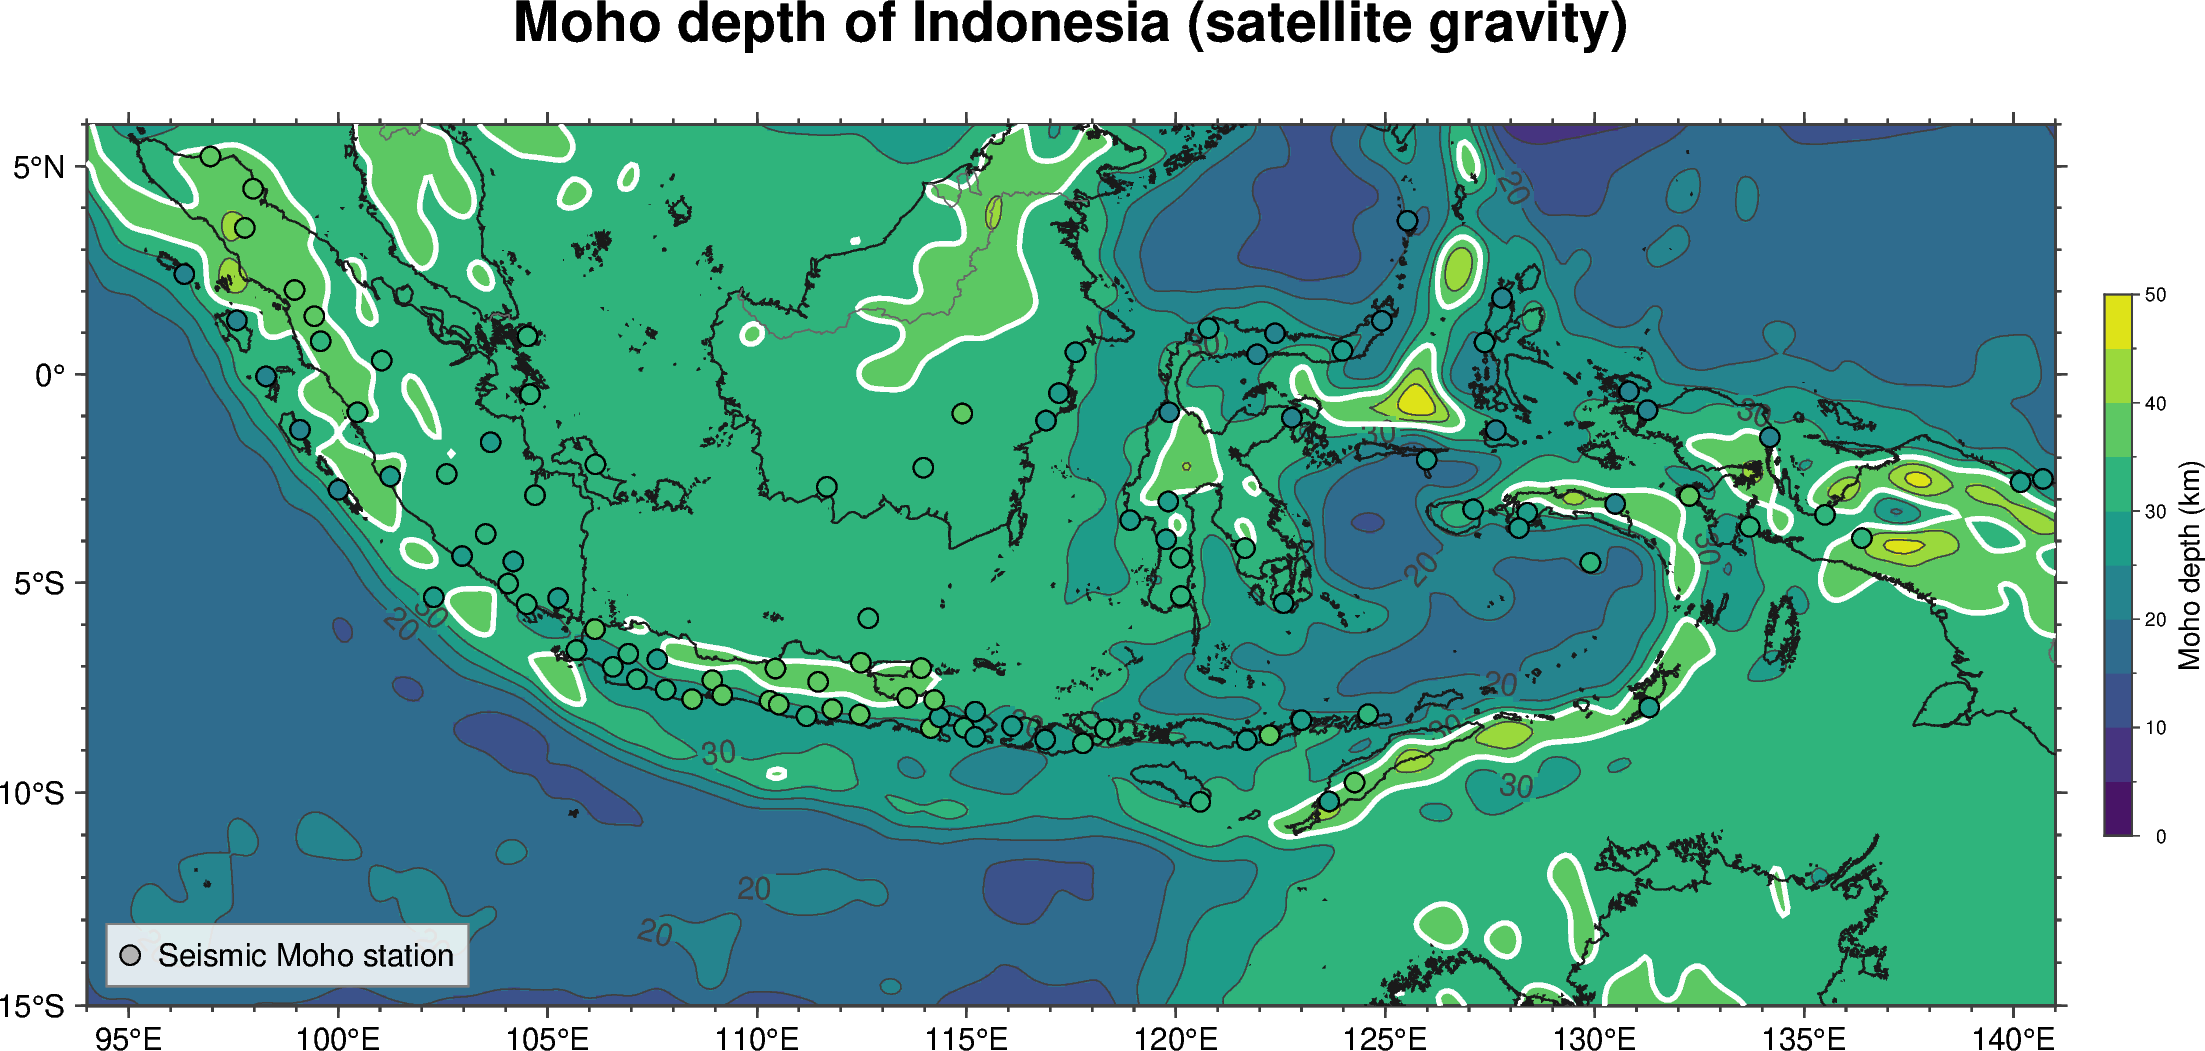
\includegraphics[width=\textwidth]{../figures/moho/moho_full_clean.png}
\caption{Estimated Moho depth of Indonesia from GOCO06s satellite gravity, with the
105 seismic stations (dots) and depth contours (35-km contour in white).}
\label{fig:moho}
\end{figure}

\begin{figure}
\centering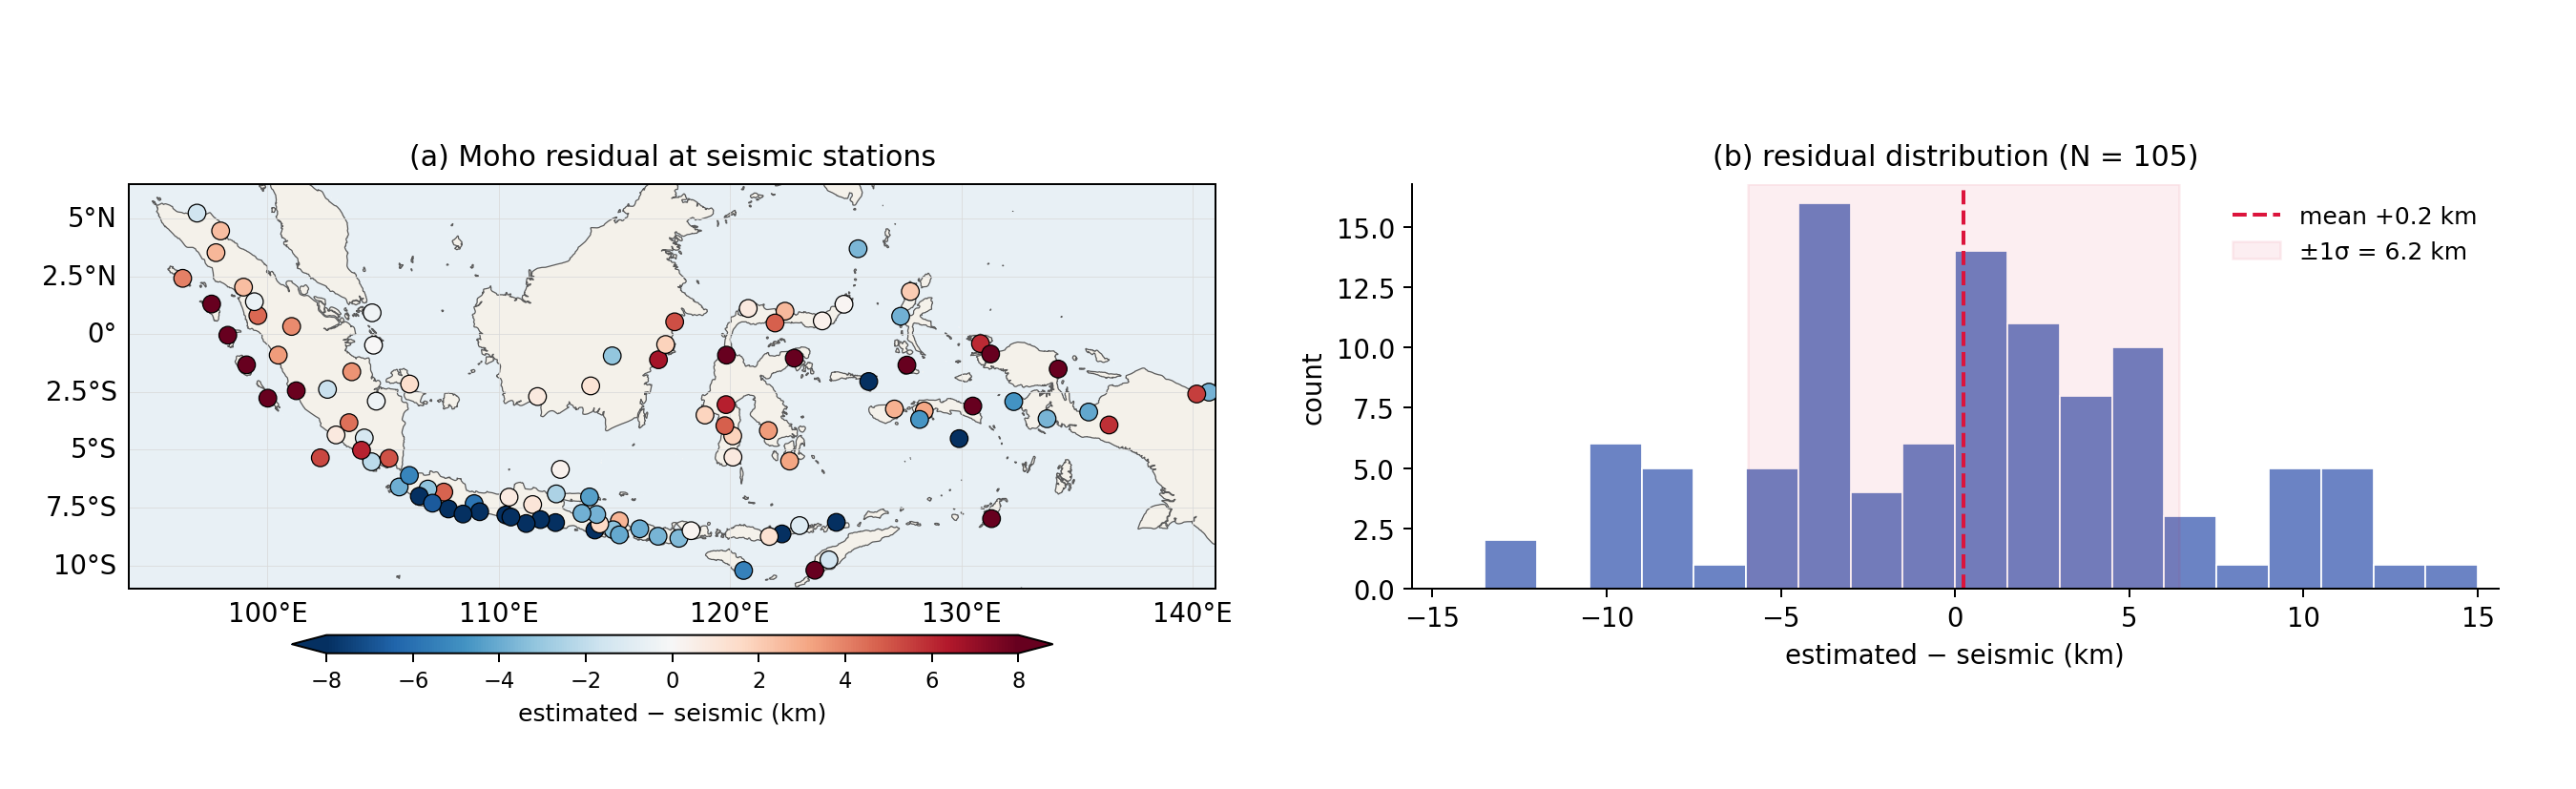
\includegraphics[width=0.8\textwidth]{../figures/moho/validation_seismic.png}
\caption{Moho residual (estimated $-$ seismic) at the 105 stations: (a) map,
(b) histogram (mean $+1.2$, std $5.8$~km).}
\label{fig:validation}
\end{figure}

\begin{figure}
\centering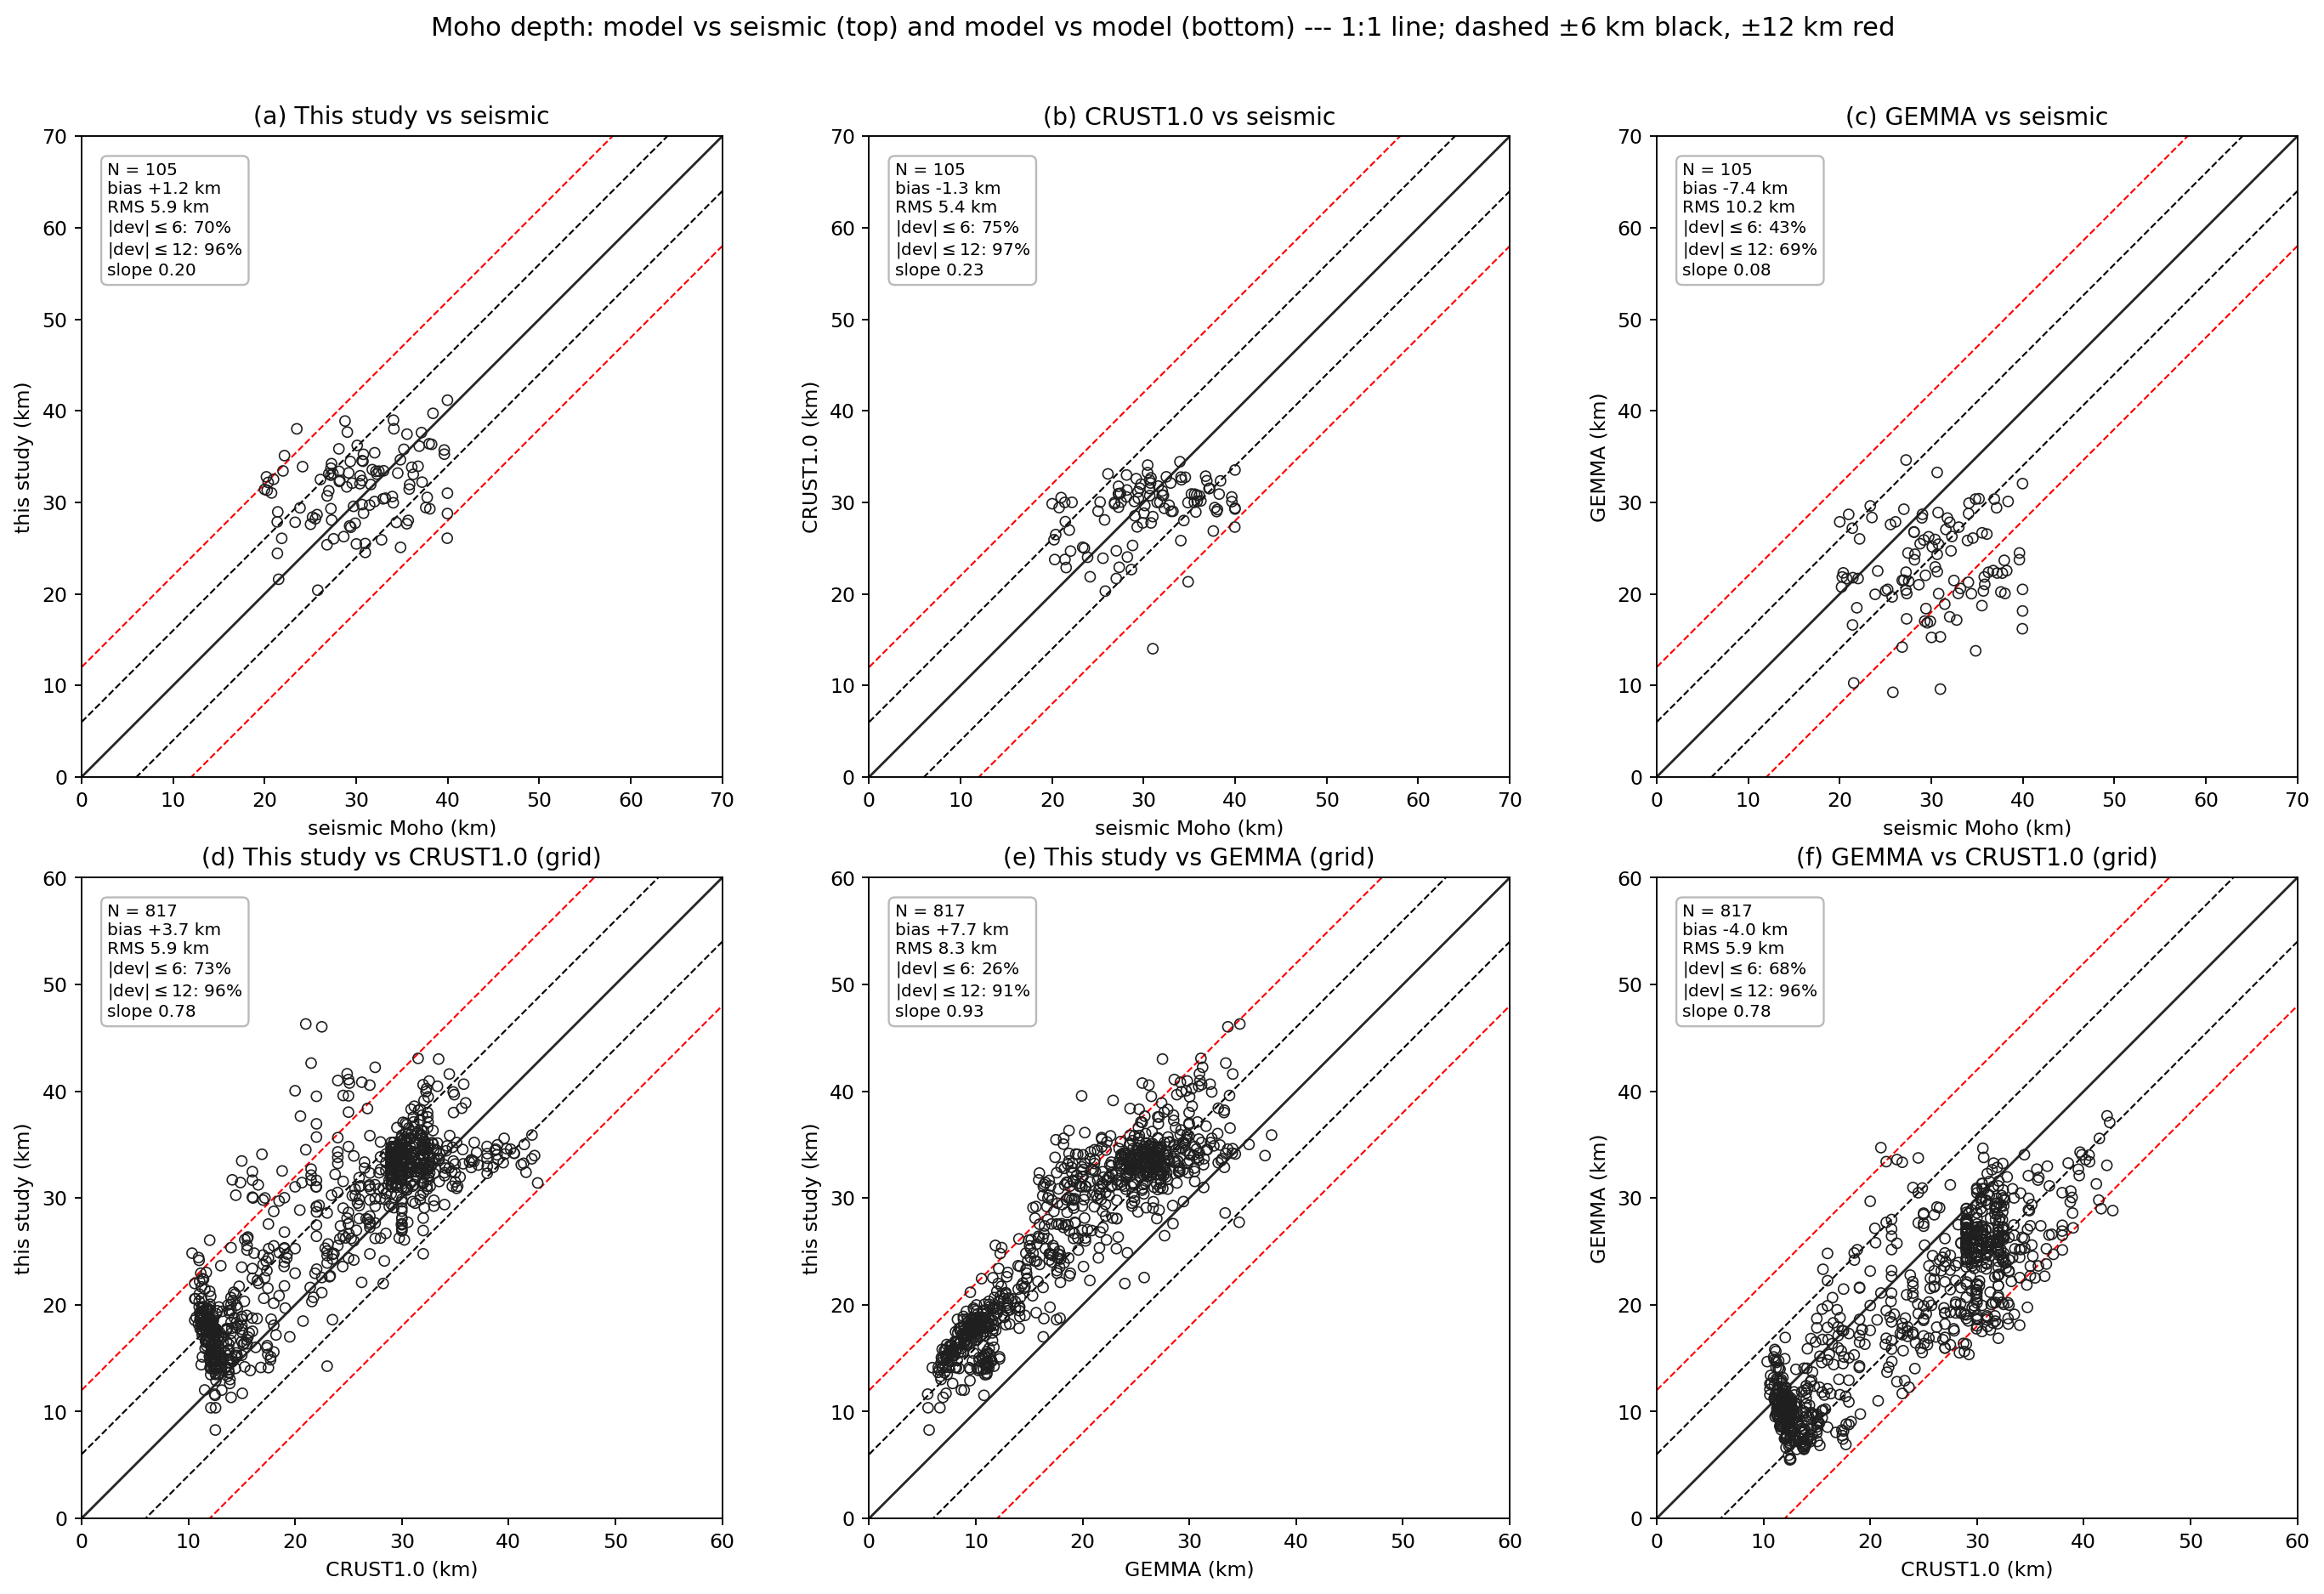
\includegraphics[width=\textwidth]{../figures/moho/scatter_vandermeijde.png}
\caption{Depth--depth comparison (after \citeA{vandermeijde2013}): open circles
against the 1:1 line, with $\pm6$~km (black dashed) and $\pm12$~km (red dashed)
deviation bands; inset: bias, RMS, per cent within $\pm6$/$\pm12$~km and slope.
Top, versus the 105 seismic depths: (a) this study, (b) CRUST1.0, (c) GEMMA.
Bottom, model versus model over the grid ($N=817$): (d) this study vs CRUST1.0,
(e) this study vs GEMMA, (f) GEMMA vs CRUST1.0. Against point seismic, this study
(slope 0.20) and CRUST1.0 (slope 0.23) show the same amplitude compression;
grid-to-grid, this study tracks CRUST1.0 (slope 0.78) and shares GEMMA's pattern
(slope 0.93), but GEMMA is $\sim8$~km too shallow.}
\label{fig:scatter}
\end{figure}

\begin{figure}
\centering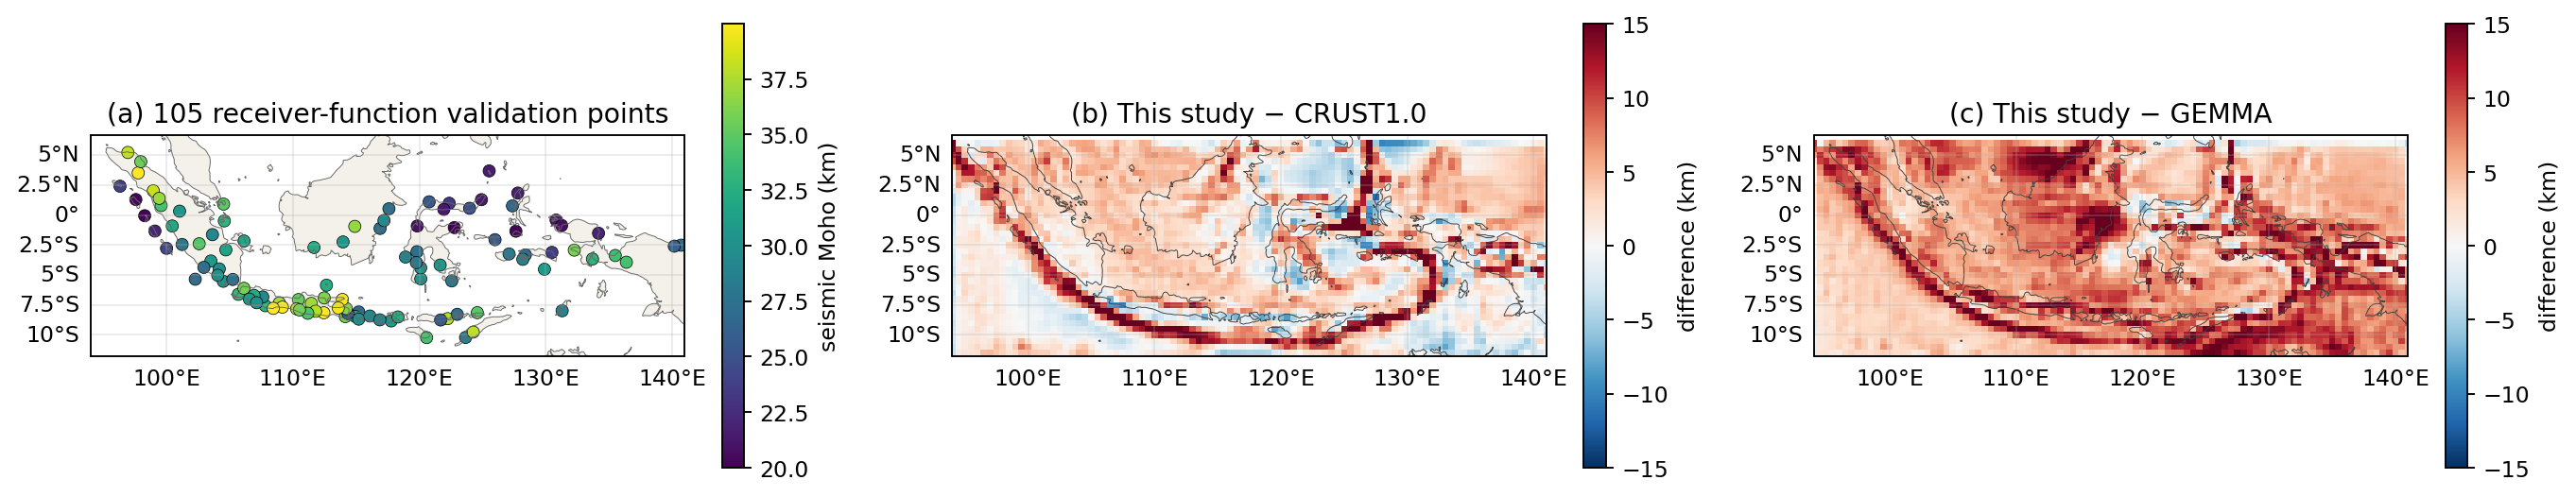
\includegraphics[width=\textwidth]{../figures/moho/compare_global_models.png}
\caption{(a) The 105 RF stations coloured by seismic Moho depth. (b) This study
$-$ CRUST1.0: agreement within $\pm5$~km inland, deeper only along the Sunda--Java
trench. (c) This study $-$ GEMMA: our model is 5--10~km deeper almost everywhere,
reflecting GEMMA's systematic shallow bias over Indonesia.}
\label{fig:compare}
\end{figure}

\begin{table}
\caption{Difference (model $-$ seismic) at the 105 RF stations. IQR: interquartile
range; $\pm5$/$\pm10$: per cent of stations within $\pm5$/$\pm10$~km.}
\label{tab:compare}
\centering
\begin{tabular}{lccccccc}
\hline
Model & Mean & Median & Std & IQR & RMS & $r$ & $\pm10$~km\\
      & (km) & (km)   & (km)& (km)& (km)&     & (\%)\\
\hline
This study & $+1.2$ & $+1.2$ & 5.8 & 6.9 & 5.9 & 0.28 & 89\\
CRUST1.0   & $-1.3$ & $-1.2$ & 5.3 & 7.5 & 5.4 & 0.36 & 94\\
GEMMA      & $-7.4$ & $-6.5$ & 7.1 & 9.5 & 10.2 & 0.08 & 64\\
\hline
\end{tabular}
\end{table}

\end{document}
